\documentclass[article, 12pt, oneside, a4paper, english, brazil, section=TITLE]{abntex2}
\usepackage{abntartigo}
\addbibresource{referencias.bib}
\graphicspath{{../reports/figures/05_model_interpretation/}}

\titulo{Previsão da variação do valor de mercado de jogadores das \textit{Big Five} europeias com
  aprendizado de máquina explicável: evidências para a estratégia \textit{buy-low/sell-high}}
\adicionarautor{Álvaro Teixeira de Araújo}
\adicionarautor{Renan Almeida Ferreira}
\orientacao{Orientadora}{Profa. Ma. Maria Eva Clemencia Fonseca Castro Silva}
\palavraschave{valor de mercado; futebol; aprendizado de máquina; SHAP; previsão.}

\begin{document}

\imprimircabecalho

\begin{resumo}
Clubes que adotam o modelo de \textit{player trading} precisam identificar, antes do mercado, os atletas que vão se valorizar.
Este estudo avalia em que medida a variação do valor de mercado de jogadores de linha das cinco principais ligas europeias pode ser prevista uma e duas temporadas à frente ($T+1$ e $T+2$) com informação disponível ao fim da temporada de referência.
A amostra reúne 13.748 observações jogador–temporada de 5.007 atletas, de 2018/19 a 2024/25, restritas aos 90\% de menor valor e a quem jogou ao menos 90 minutos, com dados do FBref, do Understat, do Sofascore e do Transfermarkt.
Foram comparados seis algoritmos e arquiteturas globais e segmentadas por idade e posição, sob validação em janela expandida e com o teste de $T+1$ (2024/25) pré-registrado.
No teste, o modelo explicou 33\% da variância do log-retorno em $T+1$ e 37\% em $T+2$, e 67\% dos atletas do decil superior previsto valorizaram-se o bastante para cobrir custos de transação de 10\% na compra e na venda, contra 22\% na média.
O desempenho em campo agregou poder preditivo ao próprio Transfermarkt, sobretudo no auge da carreira, mas a idade foi o principal determinante, e modelos separados por categoria não superaram um modelo único.
Em simulação líquida de custos, as carteiras do modelo superaram o acaso, o \textit{momentum} e a compra dos atletas mais jovens em todas as temporadas.
O aprendizado de máquina explicável mostrou-se útil para triar e ordenar oportunidades, e não para precificar atletas individualmente.
\end{resumo}

\section{Introdução}

O mercado de transferências do futebol europeu combina inflação dos valores negociados, endividamento dos clubes e regras de sustentabilidade financeira cada vez mais rigorosas \cite{hill2026}.
Nesse ambiente, clubes de médio porte e clubes formadores adotam o modelo de \textit{player trading}: adquirir atletas subavaliados, desenvolvê-los e revendê-los com ágio, segundo a lógica \textit{buy-low/sell-high} que organizações como o FC Midtjylland e o TSG Hoffenheim associam ao uso sistemático de dados \cite{muller2017}.

A execução dessa estratégia depende de uma previsão: quais atletas, disponíveis hoje a preços compatíveis com o orçamento, valerão mais em uma ou duas temporadas.
A literatura de valoração concentra-se, porém, em estimar o nível atual do valor de mercado ou do preço de transferência (\textit{nowcasting}), por regressão \cite{muller2017} ou por aprendizado de máquina \cite{mchale2023,khalife2025}.
Estimar bem o nível não garante prever a variação: um modelo que reproduz o valor publicado pelo Transfermarkt herda a inércia da avaliação da plataforma, sujeita a ancoragem e a cascatas de informação \cite{herm2014,coates2022}.

Dois problemas metodológicos agravam essa lacuna.
O primeiro é a avaliação: com dados longitudinais, a validação cruzada aleatória e a reutilização do conjunto de teste durante o desenvolvimento produzem métricas otimistas \cite{kaufman2011,kapoor2023}.
O segundo é a opacidade: quem decide a contratação precisa saber por que um atleta é recomendado, o que motiva explicações aditivas como o SHAP \cite{lundberg2017}.

Este artigo tem como objetivo prever a variação absoluta e percentual do valor de mercado, uma e duas temporadas à frente ($T+1$ e $T+2$), dos jogadores de linha das cinco principais ligas europeias (\textit{Big Five}) situados entre os 90\% de menor valor e com ao menos 90 minutos na temporada de referência, e avaliar se essas previsões sustentam decisões de recrutamento e revenda.
As contribuições são quatro: tratar o problema como previsão temporal estrita, com o teste final de $T+1$ (2024/25) pré-registrado; testar se o desempenho em campo agrega informação ao que o Transfermarkt já incorpora; submeter a teste formal a segmentação em 12 categorias de idade e posição, em lugar das nove de \textcite{khalife2025}; e avaliar as previsões como regra de decisão, líquida de custos de transação, com explicações SHAP.

\section{Revisão da literatura}

\subsection{Desempenho, ciclo de vida e valor de mercado}

A revisão sistemática de \textcite{franceschi2024} organiza os determinantes do valor de jogadores em características do atleta (idade, posição, desempenho e experiência), do contrato, do clube e de popularidade.
A idade mantém relação em U invertido com a remuneração e o valor \cite{frick2007}, e o desempenho é medido cada vez mais por métricas de eventos por 90 minutos.
No topo da distribuição, porém, a economia das superestrelas \cite{rosen1981,lucifora2003} gera prêmios desproporcionais ao desempenho, e \textcite{muller2017} observaram que modelos baseados em dados superam as estimativas da comunidade justamente abaixo do percentil 90 dos valores.

\textcite{hill2026} distinguem o valor de um atleta, associado ao desempenho esportivo em relação ao custo, do preço, resultado de uma negociação influenciada pelo tempo de contrato, pela liquidez dos clubes e pelo poder de barganha.
Como o fluxo de caixa de um único atleta não é isolável e o valor residual se anula ao fim do contrato, os autores adaptam ao futebol as tipologias de valoração relativa e probabilística de \textcite{damodaran2012}, arcabouço em que este estudo se insere.

\subsection{Transfermarkt e a sabedoria das multidões}

Na ausência de preços contínuos de transação, o valor publicado pelo Transfermarkt tornou-se a \textit{proxy} padrão da literatura.
Sua lógica remete à sabedoria das multidões, que exige diversidade, independência, descentralização e agregação dos julgamentos \cite{surowiecki2004}.
\textcite{herm2014} mostraram, contudo, que a plataforma opera pelo \enquote{princípio do juiz}: avaliadores designados ponderam propostas de usuários que conhecem as estimativas anteriores, o que favorece a ancoragem \cite{tversky1974} e as cascatas de informação \cite{bikhchandani1992}.
Ainda assim, esses valores correlacionam-se com os preços de transferência e antecipam resultados esportivos \cite{herm2014,peeters2018}, e \textcite{coates2022} examinam sua relação com os valores efetivamente pagos.
Para um estudo de previsão, o valor do Transfermarkt é o alvo observável, mas a trajetória das suas revisões pode carregar inércia própria, que precisa ser separada da informação de desempenho.

\subsection{Aprendizado de máquina na valoração de atletas}

\textcite{muller2017} estimaram valores de mercado por regressão multinível com desempenho e popularidade; \textcite{mchale2023}, valores de transferência com métricas avançadas e aprendizado de máquina; e \textcite{khalife2025} segmentaram modelos de \textit{gradient boosting} em nove grupos, cruzando três faixas etárias e três posições, e mostraram que incluir o potencial projetado do atleta eleva a precisão média dos modelos de 74\% para 84\%, com queda para 59\% entre atacantes acima de 30 anos.
Esses valores referem-se ao nível do valor, e não à sua variação futura, alvo muito mais ruidoso.

Com dados longitudinais, a avaliação exige validação que respeite a ordem temporal \cite{bergmeir2018,cerqueira2020}, barreiras contra o vazamento de informação futura \cite{kaufman2011} e comparações que considerem a incerteza amostral das diferenças de erro \cite{diebold1995,hansen2011}.
O vazamento e a seleção de modelos no próprio conjunto de teste inflam resultados publicados \cite{kapoor2023}, e o pré-registro do protocolo de análise é uma das respostas a esse problema \cite{nosek2018}.

\subsection{Explicabilidade na tomada de decisão}

Os valores SHAP decompõem cada previsão em contribuições aditivas das variáveis, com base nos valores de Shapley da teoria dos jogos cooperativos \cite{lundberg2017}, e têm algoritmo exato e eficiente para conjuntos de árvores \cite{lundberg2020}.
No recrutamento, permitem verificar se uma recomendação decorre do desempenho, da idade, do preço ou do contexto do clube.
Duas ressalvas orientam o seu uso: as explicações descrevem o modelo, e não relações causais, e variáveis correlacionadas dividem entre si a contribuição atribuída.

\section{Problema e objetivos}

Para um clube que opera \textit{player trading}, o problema não é saber quanto um atleta vale hoje, mas se ele vai se valorizar o bastante, entre a compra e a revenda, para pagar a operação.
A pergunta de pesquisa é: em que medida a variação do valor de mercado, absoluta ($\Delta V$) e percentual ($\Delta V\%$), em $T+1$ e $T+2$, dos 90\% jogadores de linha mais baratos das \textit{Big Five} com ao menos 90 minutos em $T$ pode ser prevista com informação disponível em $T$, de modo a fundamentar decisões de recrutamento e revenda?

O objetivo geral é desenvolver e validar modelos de aprendizado de máquina para essa previsão e avaliá-los como instrumento de decisão.
Os objetivos específicos são:

\begin{alineas}
  \item integrar e verificar dados de desempenho, demografia, contexto do clube e valor de mercado dos atletas elegíveis;
  \item treinar e comparar algoritmos lineares e de conjuntos de árvores, em arquiteturas globais e segmentadas, sob validação temporal sem vazamento;
  \item identificar, com SHAP, os determinantes da valorização nas 12 categorias de idade e posição;
  \item avaliar o desempenho econômico de uma estratégia \textit{buy-low/sell-high} baseada nas previsões, líquida de custos.
\end{alineas}

As hipóteses e seus critérios de decisão foram fixados no protocolo pré-registrado:

\begin{alineas}[label=H\arabic*:]
  \item o desempenho em $T$ tem poder preditivo incremental além do Transfermarkt (nível e trajetória do valor) e da idade;
  \item a matriz de 12 categorias (4~×~3) supera a de nove categorias (3~×~3) de \textcite{khalife2025} e o modelo global;
  \item atletas subavaliados pelo desempenho valorizam-se mais, premissa da compra a preço baixo;
  \item a carteira selecionada pelo modelo supera heurísticas e o acaso, líquida de custos e incluindo os atletas que saem da base;
  \item o desempenho pesa mais na valorização no auge da carreira do que entre os veteranos.
\end{alineas}

\section{Diferencial do estudo}

O estudo difere da literatura de referência no objeto, pois prevê a variação do valor, e não o nível atual; no rigor da avaliação, com janela expandida, teste pré-registrado, inferência por \textit{clusters} e correção para comparações múltiplas; e no uso, pois avalia as previsões como regra de compra, líquida de custos, e testa as premissas das especificações, inclusive as que os dados não confirmaram.
O Quadro~\ref{qua:diferencial} sintetiza essas diferenças.

\begin{quadro}[htbp]
  \caption{Contribuições do estudo frente à literatura de referência}
  \label{qua:diferencial}
  \begin{tabularx}{\textwidth}{|>{\hsize=.62\hsize}L|>{\hsize=1.1\hsize}L|>{\hsize=1\hsize}L|>{\hsize=1.28\hsize}L|}
    \hline
    Estudo & Abordagem & Limitação para o \textit{player trading} & Contribuição deste estudo \\
    \hline
    \textcite{muller2017} & Regressão multinível do valor com desempenho e popularidade & Estima o nível do valor (\textit{nowcasting}) & Prevê a variação em $T+1$ e $T+2$ nos 90\% de menor valor \\
    \hline
    \textcite{coates2022} & Avaliação coletiva do Transfermarkt e valores de transferência & Não propõe um previsor alternativo & Testa se o desempenho agrega informação ao Transfermarkt (H1) \\
    \hline
    \textcite{mchale2023} & Aprendizado de máquina com métricas avançadas de desempenho & Estima o nível, sem avaliar decisões & Avalia carteiras com custos e intenção de tratar (H4) \\
    \hline
    \textcite{khalife2025} & \textit{Gradient boosting} segmentado em nove grupos (3~×~3) & Queda de precisão nos atacantes acima de 30 anos & Testa formalmente as matrizes 4~×~3 e 3~×~3 e o modelo global (H2) \\
    \hline
    \textcite{hill2026} & Tipologias de valoração de Damodaran aplicadas ao futebol & Proposta conceitual, sem validação empírica & Operacionaliza a valoração relativa e probabilística com previsões e intervalos calibrados \\
    \hline
  \end{tabularx}
  \fonte{Elaboração própria.}
\end{quadro}

\section{Verificação dos dados}

\subsection{Fontes e integração}

O FBref fornece a espinha dorsal da amostra (minutos, jogos, gols, assistências, finalizações e cartões).
Como a plataforma retirou, em janeiro de 2026, as métricas avançadas licenciadas da Opta, inclusive das temporadas passadas, o vetor tático-técnico foi completado com o Understat (gols e assistências esperados) e o Sofascore (passes, dribles, duelos, desarmes, grandes chances e nota).
O Transfermarkt fornece os valores de mercado datados, o perfil dos atletas e as transferências.
Foram coletadas as temporadas de 2018/19 a 2024/25, além de 2017/18 para as defasagens, num total de 22.419 registros jogador–clube–temporada.

Na ausência de identificador comum, os registros foram pareados por resolução de entidades: normalização dos nomes, similaridade de Levenshtein e de Jaro-Winkler, restrições de ano de nascimento e de minutagem e 45 correspondências manuais.
O pareamento com o Transfermarkt alcançou 99,94\% do universo-alvo.
O valor em $T$ ($V_T$) é a última avaliação publicada até 30 de junho do ano de término da temporada, com defasagem máxima de 183 dias, e $V_{T+1}$ e $V_{T+2}$ seguem a mesma regra um e dois anos depois; assim, nenhuma variável explicativa incorpora informação posterior à data da decisão.

\subsection{Amostra}

A Tabela~\ref{tab:funil} apresenta o funil amostral, que resulta em 13.748 observações jogador–temporada de 5.007 atletas.

\begin{table}[htbp]
  \caption{Funil amostral (2018/19 a 2024/25)}
  \label{tab:funil}
  \begin{tabularx}{\textwidth}{Lrrr}
    \toprule
    Etapa & Observações & Atletas & Retenção \\
    \midrule
    Registros do FBref (jogador–clube–temporada) & 19.727 & 6.643 & — \\
    Jogador–temporada & 18.808 & 6.643 & 95,3\% \\
    Pareados com o Transfermarkt & 18.763 & 6.609 & 99,8\% \\
    Exclusão de goleiros & 17.339 & 6.101 & 92,4\% \\
    Minutagem de ao menos 90 minutos em $T$ & 15.286 & 5.138 & 88,2\% \\
    Com $V_T$ observado & 15.184 & 5.088 & 99,3\% \\
    Corte no percentil 90 de $V_T$ & 13.748 & 5.007 & 90,5\% \\
    \bottomrule
  \end{tabularx}
  \fonte{Elaboração própria com dados de FBref e Transfermarkt.}
\end{table}

Três verificações merecem destaque.
O percentil 90 de $V_T$, calculado por temporada, situa-se entre €~27 e €~32 milhões, acima dos €~18 milhões de \textcite{muller2017}, que correspondem ao percentil 81 desta amostra; o corte é assimétrico, pois exclui 21\% das observações da Premier League e 4\% das da Ligue~1.
O filtro de 90 minutos remove sobretudo jovens (23\% dos atletas de 16 a 23 anos), de modo que as conclusões sobre essa faixa valem para jovens já integrados ao elenco principal.
As 12 categorias têm tamanhos desiguais, de 2.233 observações (defensores de 24 a 28 anos) a 341 (atacantes de 33 anos ou mais), com faixas definidas pelos anos completos em 30 de junho (16–23, 24–28, 29–32 e 33 anos ou mais), o que resolve a sobreposição dos rótulos das especificações aos 28 anos.

\subsection{Variáveis-alvo}

A variação percentual é extremamente assimétrica: nas temporadas de desenvolvimento, a mediana de $\Delta V\%$ em $T+1$ é −20,0\% e a média, +5,8\%, com assimetria de 19,8.
Por isso, o alvo de treino é o log-retorno (assimetria de 1,10), e as previsões são reconvertidas para $\Delta V\%$ e $\Delta V$.
Cerca de um em cada quatro atletas se valoriza por ano; a exceção é 2018/19, cujo $V_{T+1}$ coincide com a revisão extraordinária de abril de 2020, na pandemia, quando 82\% dos atletas perderam valor.
A ausência do alvo concentra-se nos veteranos (de 22\% a 26\% sem $V_{T+2}$ aos 33 anos ou mais), um viés de sobrevivência tratado na simulação por intenção de tratar.

\section{Metodologia e design do modelo}

\subsection{Variáveis}

Para o atleta $i$ na temporada $T$, o alvo no horizonte $k \in \{1, 2\}$ é o log-retorno do valor, definido na equação~\eqref{eq:alvo}:
\begin{equation}
  y_{i,k} = \ln\left(\frac{V_{i,T+k}}{V_{i,T}}\right), \qquad \Delta V\%_{i,k} = e^{y_{i,k}} - 1
  \label{eq:alvo}
\end{equation}

O vetor explicativo reúne 108 variáveis medidas até 30 de junho de $T$: demografia (idade decimal e seu quadrado, altura e pé preferido), mercado ($\log V_T$ e peso no valor do elenco), contexto do clube (desempenho da equipe, promoção, rebaixamento e participação europeia), dinâmica do valor (revisões recentes e distância ao pico), defasagens (\textit{momentum} e desempenho em $T-1$) e 52 métricas de desempenho por 90 minutos e de eficiência, além de liga, faixa etária e posição.

Como as taxas de quem joga pouco são dominadas pelo acaso, cada métrica foi encolhida para a média da sua posição na temporada por métodos empírico-bayesianos \cite{efron1975}: nas contagens, pelo estimador gama–Poisson de \textcite{clayton1987}, na equação~\eqref{eq:shrink}, em que $c_i$ é a contagem, $e_i$ são os minutos divididos por 90 e $\alpha$ e $\beta$ são parâmetros \textit{a priori} estimados por momentos; nos percentuais, pelo análogo beta–binomial.
Encolhidas, as métricas tornaram-se mais estáveis: a correlação de postos entre $T-1$ e $T$ aumentou em 50 das 52 métricas.
\begin{equation}
  \tilde{r}_i = \frac{\alpha + c_i}{\beta + e_i}
  \label{eq:shrink}
\end{equation}

Duas variáveis sintetizam a premissa \textit{buy-low}.
O valor justo é a previsão de $\ln V_T$ pelo desempenho, pela idade, pela posição e pelo contexto, ajustada por \textit{gradient boosting} com validação cruzada dentro de cada temporada ($R^2$ fora da dobra de 0,79); o \textit{gap} de avaliação é a diferença entre $\ln V_T$ e o valor justo, negativa para atletas subavaliados.
O tempo restante de contrato ficou fora do vetor, porque o Transfermarkt publica apenas o contrato vigente na data da coleta, e sua reconstrução em $T$ depende de eventos posteriores, o que antecipa o desfecho.

\subsection{Validação temporal e pré-registro}

A validação usa janela expandida: cada dobra treina com as temporadas anteriores e testa na seguinte.
Há seis dobras em $T+1$, com testes de 2019/20 a 2024/25, e quatro em $T+2$, com purga de uma temporada entre treino e teste, já que o alvo de $T+2$ só é conhecido duas temporadas depois.
Imputação, winsorização e padronização são ajustadas dentro de cada dobra.

O teste final de $T+1$ (2024/25, com alvo em 30 de junho de 2026) foi pré-registrado \cite{nosek2018}: as decisões de modelagem foram tomadas nas dobras de desenvolvimento, com esses alvos ocultos, e o protocolo (\textit{hash} dos dados e do código, variáveis, dobras, hiperparâmetros, arquitetura e critérios das hipóteses) foi versionado antes da revelação, condicionada à verificação automática de que ele era idêntico ao reproduzido.
O teste de $T+2$ (2023/24) é semi-independente, pois foi consultado em versões anteriores do estudo.

\subsection{Algoritmos, arquiteturas e otimização}

Foram comparados uma referência ingênua (mediana do treino por categoria), mínimos quadrados ordinários, Ridge \cite{hoerl1970}, floresta aleatória \cite{breiman2001}, XGBoost \cite{chen2016} e CatBoost \cite{prokhorenkova2018}.
O modelo principal é um \textit{ensemble} fixado \textit{a priori}, a média simples de CatBoost, XGBoost e Ridge, pois combinações simples tendem a superar pesos estimados \cite{smith2009}.
Para testar a segmentação, os modelos foram ajustados em três arquiteturas: global, com idade e posição como variáveis; segmentada, com um modelo por categoria nas matrizes 4~×~3 e 3~×~3; e \textit{pooling} parcial, que combina o segmento $c$ e o modelo global com peso crescente no tamanho $n_c$ do segmento, conforme a equação~\eqref{eq:pool}:
\begin{equation}
  \hat{y}_i = w_c\,\hat{y}^{\mathrm{seg}}_i + (1 - w_c)\,\hat{y}^{\mathrm{glob}}_i, \qquad w_c = \frac{n_c}{n_c + \kappa}
  \label{eq:pool}
\end{equation}

A regra pré-declarada só substituiria o \textit{ensemble} global por uma alternativa com erro de validação menor e diferença significativa após a correção de Holm.
Os hiperparâmetros foram escolhidos por otimização bayesiana com processo gaussiano \cite{snoek2012}, com 20 avaliações nos modelos globais e minimização da raiz do erro quadrático médio (RMSE) das três últimas dobras de validação; no \textit{boosting}, a taxa de aprendizado foi fixada em 0,05, e o número de árvores, definido por parada antecipada temporal.

\subsection{Magnitude e incerteza}

Uma camada de magnitude converte o log-retorno previsto em $\Delta V\%$, com recalibração linear (parâmetros $a$ e $b$) e fator de \textit{smearing} de \textcite{duan1983} por faixa etária, $f_g$, estimados apenas com as dobras anteriores, conforme a equação~\eqref{eq:smear}.
Intervalos de previsão de 80\% foram obtidos por regressão quantílica com CatBoost e conformalização sequencial \cite{romano2019}.
\begin{equation}
  \widehat{\Delta V\%}_i = f_g \exp\left(a + b\,\hat{y}_i\right) - 1
  \label{eq:smear}
\end{equation}

\subsection{Inferência, explicabilidade e avaliação da decisão}

As incertezas foram estimadas por \textit{bootstrap} de \textit{clusters} clube~×~temporada, pois atletas do mesmo clube compartilham choques \cite{cameron2008}.
Os modelos foram comparados por teste pareado de perdas do tipo Diebold–Mariano, com erro-padrão agrupado e correção para pequenas amostras \cite{diebold1995,harvey1997}, correção de \textcite{holm1979} e conjunto de confiança de modelos \cite{hansen2011}.
A H1 foi testada por ablação de blocos de variáveis \cite{lei2018}.
As previsões do \textit{ensemble} foram explicadas por valores SHAP, que decompõem cada previsão em um valor-base $\phi_0$ e contribuições aditivas $\phi_{ij}$ das $M$ variáveis, conforme a equação~\eqref{eq:shap}, com o algoritmo exato para árvores e a forma fechada linear no Ridge.
\begin{equation}
  \hat{y}_i = \phi_0 + \sum_{j=1}^{M} \phi_{ij}
  \label{eq:shap}
\end{equation}

Por fim, a simulação \textit{buy-low/sell-high} compra, em cada temporada de teste, os 10\% de candidatos com maior retorno esperado e os avalia em $T+k$.
No cenário principal, compra-se por $V_T(1 + c_b)$ e vende-se por $V_{T+k}(1 - c_v)$, com $c_b = c_v = 10\%$, e quem sai da base vale zero (intenção de tratar).
Uma operação só é lucrativa se a valorização superar o ponto de equilíbrio dos custos, dado pela equação~\eqref{eq:breakeven} e igual a 22,2\% no cenário principal.
Esse limiar define a \enquote{valorização significativa} na avaliação das previsões como regra de compra, feita pela área sob a curva ROC, ou AUC \cite{fawcett2006}, pelo escore de Brier \cite{brier1950} e por probabilidades calibradas com regressão isotônica \cite{zadrozny2002}.
\begin{equation}
  \Delta V\% > \frac{1 + c_b}{1 - c_v} - 1
  \label{eq:breakeven}
\end{equation}

\section{Resultados e discussão}

\subsection{Desempenho preditivo}

A variação futura do valor é parcialmente previsível, como resume a Tabela~\ref{tab:teste}.
No teste pré-registrado, o \textit{ensemble} explica 33\% da variância do log-retorno em $T+1$ (IC 95\%: 29\% a 36\%) e reduz a RMSE em 19\% frente à hipótese de valor constante; em $T+2$, a arquitetura final explica 37\%.
O desempenho cresce com a janela de treino, de $R^2$ de 0,18 na primeira dobra de $T+1$ a 0,29 na última de desenvolvimento, tendência que o teste de 2024/25 continua.
Árvores e modelos lineares empatam: o \textit{ensemble} é o único modelo sempre presente no conjunto de confiança, mas sua vantagem sobre Ridge, XGBoost e floresta aleatória não é significativa, e os hiperparâmetros-padrão produziram o mesmo erro que os otimizados.
O sinal está nas variáveis, e não no algoritmo.

\begin{table}[htbp]
  \caption{Desempenho no teste final, por modelo (log-retorno)}
  \label{tab:teste}
  \begin{tabularx}{\textwidth}{Lrrrrrr}
    \toprule
    Modelo & RMSE $T+1$ & $R^2$ $T+1$ & $\rho$ $T+1$ & RMSE $T+2$ & $R^2$ $T+2$ & $\rho$ $T+2$ \\
    \midrule
    Sem variação ($V_{T+k} = V_T$) & 0,673 & −0,03 & — & 0,992 & −0,17 & — \\
    Mediana por categoria & 0,614 & 0,14 & 0,46 & 0,789 & 0,26 & 0,52 \\
    Mínimos quadrados & 0,551 & 0,31 & 0,53 & 0,731 & 0,37 & 0,58 \\
    Ridge & 0,544 & 0,33 & 0,56 & 0,728 & 0,37 & 0,59 \\
    Floresta aleatória & 0,547 & 0,32 & 0,55 & 0,733 & 0,36 & 0,60 \\
    XGBoost & 0,546 & 0,32 & 0,55 & 0,728 & 0,37 & 0,60 \\
    CatBoost & 0,548 & 0,32 & 0,55 & 0,730 & 0,37 & 0,60 \\
    \textit{Ensemble} & 0,543 & 0,33 & 0,56 & 0,724 & 0,38 & 0,60 \\
    \textit{Pooling} 3~×~3 & 0,545 & 0,33 & 0,56 & 0,728 & 0,37 & 0,60 \\
    \bottomrule
  \end{tabularx}
  \fonte{Elaboração própria.}
  \nota{$T+1$: teste pré-registrado de 2024/25 ($n = 1.952$); $T+2$: 2023/24 ($n = 1.879$). $\rho$: correlação de Spearman. Arquitetura final: \textit{ensemble} em $T+1$ e \textit{pooling} 3~×~3 em $T+2$.}
\end{table}

O maior valor do modelo está em ordenar os atletas: em todas as dobras de teste de $T+1$, 63\% do decil superior previsto se valorizou, contra 1,6\% do inferior e 27,7\% na média; no teste de 2024/25, 71\% do decil superior.
As magnitudes são menos confiáveis: a média de $\Delta V\%$ é acertada até o 9º decil, mas os maiores saltos seguem subestimados (+96\% previstos contra +194\% observados no 10º decil), e o erro absoluto mediano é de 21,5 pontos percentuais.
Os intervalos de 80\% cobriram 82\% dos casos nos dois horizontes.

\subsection{Hipóteses}

O Quadro~\ref{qua:hipoteses}, ao fim desta seção, apresenta os vereditos, obtidos com os critérios do protocolo.

A H1 é o achado central.
Retirar o desempenho em $T$ e $T-1$ e o valor justo aumenta o erro com significância nos dois horizontes, e o caminho aninhado de especificações quantifica o ganho: o $R^2$ de $T+1$ sobe de 0,251, com idade e contexto, para 0,290 com o nível de preço, 0,300 com a trajetória do valor no Transfermarkt e 0,329 com desempenho e valor justo.
Diante do desempenho, a trajetória do valor (\textit{momentum}, revisões e volatilidade) torna-se redundante.
Parte da informação de campo, portanto, ainda não está nos valores publicados, embora o ganho seja modesto, coerente com um mercado parcialmente eficiente.

A H2 contraria a inovação prevista nas especificações.
Os modelos por categoria erraram mais que o global nas duas matrizes, e o \textit{pooling} parcial apenas empatou com ele; sua vantagem nas dobras de desenvolvimento de $T+2$ não se repetiu no teste.
A queda de precisão nos atacantes veteranos relatada por \textcite{khalife2025} não se converteu em ganho da matriz 4~×~3, salvo nos atacantes de 33 anos ou mais em $T+2$, categoria pequena e sem teste formal.
A heterogeneidade por idade e posição existe (H5), mas é mais bem capturada como variável de um modelo único, que compartilha informação entre categorias.

\begin{quadro}[htbp]
  \caption{Hipóteses, critérios pré-registrados e vereditos}
  \label{qua:hipoteses}
  \begin{tabularx}{\textwidth}{|>{\hsize=1.05\hsize}L|>{\hsize=1.15\hsize}L|>{\hsize=1.15\hsize}L|>{\hsize=.65\hsize}L|}
    \hline
    Hipótese & Critério (teste final) & Resultado & Veredito \\
    \hline
    H1. O desempenho agrega ao Transfermarkt e à idade & Retirar desempenho e valor justo aumenta a RMSE (Holm $< 0,05$) & +0,011 em $T+1$ ($p < 0,001$); +0,010 em $T+2$ ($p = 0,015$) & Sustentada \\
    \hline
    H2. A matriz 4~×~3 supera a 3~×~3 e o modelo global & O conjunto de confiança contém a 4~×~3 e exclui o global e a 3~×~3 & O conjunto contém o global e as 3~×~3 nos dois horizontes & Não sustentada \\
    \hline
    H3. Subavaliados valorizam-se mais & Medianas dos quintis extremos do \textit{gap} com IC 95\% disjuntos & $T+1$: −5,9\% contra −20,0\%; em $T+2$, os ICs tocam-se em −33,3\% & Sustentada em $T+1$ \\
    \hline
    H4. A carteira do modelo supera heurísticas e o acaso & Vence o acaso nas 6 temporadas de $T+1$ e supera, na média, \textit{momentum} e juventude & 6 de 6 ($p = 0,016$); ROI de 46\% contra 9\%, 6,5\% e −19\% & Sustentada \\
    \hline
    H5. O desempenho pesa mais no auge que nos veteranos & Diferença de participação no SHAP (24–28 menos 33+) com IC acima de zero & +10,4 p.p. [10,0; 10,8] em $T+1$ e +10,5 p.p. em $T+2$ & Sustentada \\
    \hline
  \end{tabularx}
  \fonte{Elaboração própria.}
\end{quadro}

\subsection{Determinantes da valorização}

A Figura~\ref{fig:shap} mostra as 20 variáveis mais importantes em $T+1$.
A idade é o determinante isolado mais importante, com efeito quase linear, de cerca de +0,30 aos 19 anos a −0,25 aos 36.
Seguem-se o \textit{gap} de avaliação, de efeito monotônico e assimétrico (até +35\% para os mais subavaliados), e o $\log V_T$, de efeito negativo, sinal de reversão de nível compatível com a premissa \textit{buy-low}.
Por grupos, o desempenho tático-técnico responde por 29\% da explicação em $T+1$ (25\% em $T+2$), a demografia por 27\% (34\%), o contexto do clube por 11\% (7\%), com destaque para o rebaixamento, e o valor justo por 10\%.
Entre as métricas de desempenho, lideram a nota média do Sofascore e a regularidade, seguidas, nos atacantes, da presença em grandes chances, das finalizações e dos dribles.

\begin{figure}[htbp]
  \caption{Valores SHAP das 20 variáveis mais importantes para o log-retorno em $T+1$}
  \label{fig:shap}
  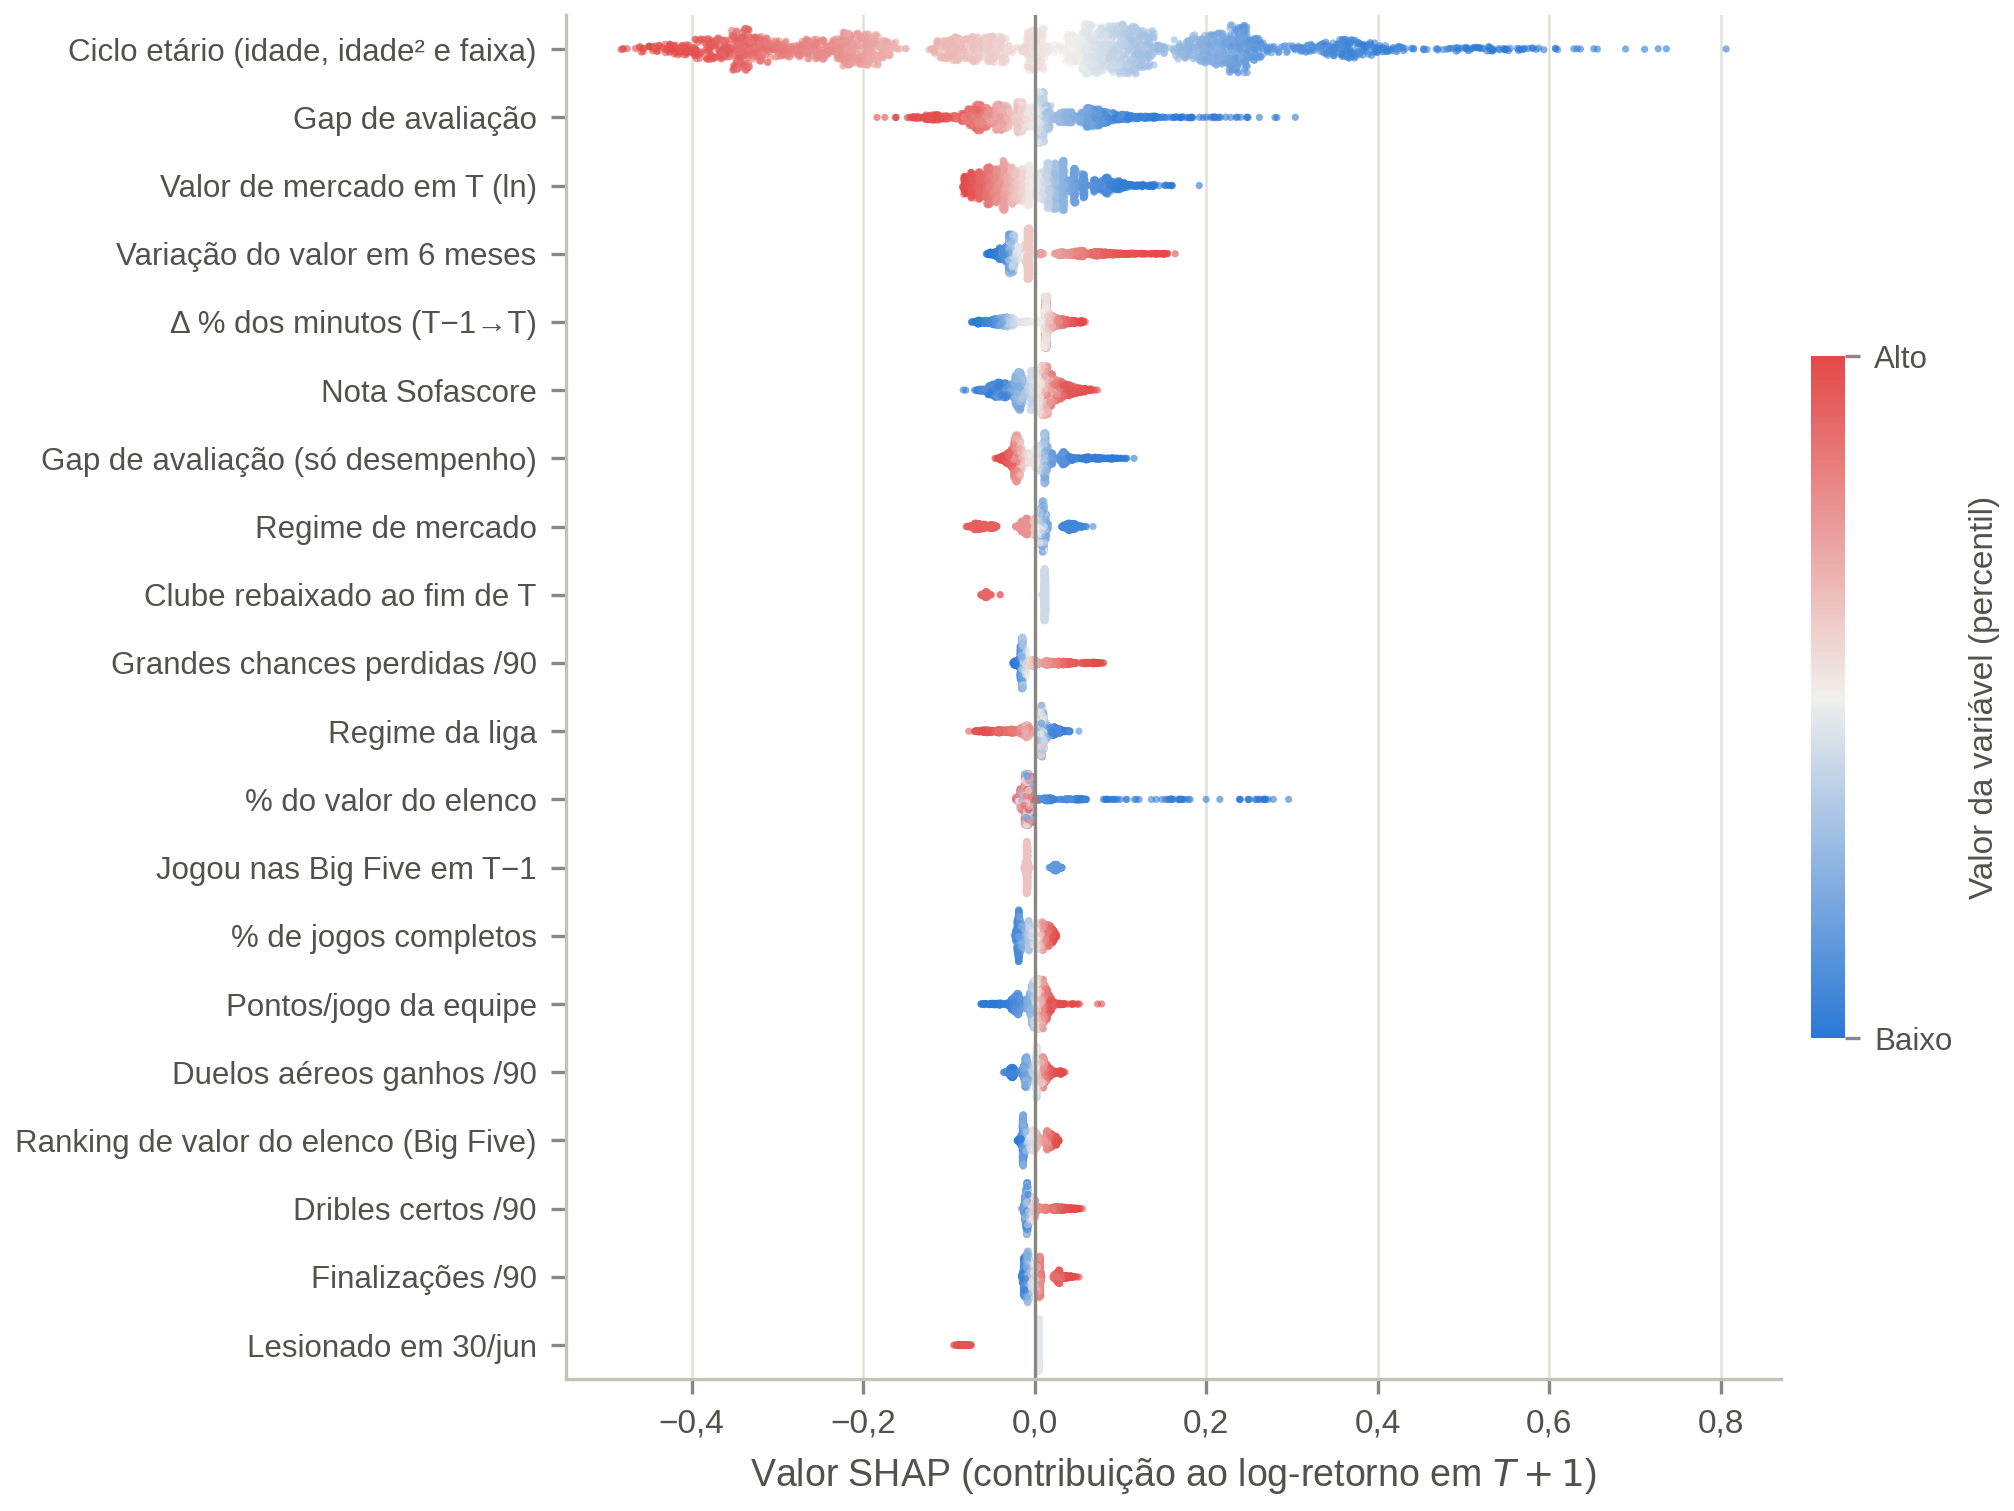
\includegraphics[width=\textwidth]{fig01_shap_beeswarm_T1.png}
  \fonte{Elaboração própria com dados de FBref, Understat, Sofascore e Transfermarkt.}
  \nota{Cada ponto é uma observação atleta–temporada; a cor indica o valor da variável.}
\end{figure}

A Figura~\ref{fig:grupos} detalha a participação dos grupos nas 12 categorias.
No auge, dos 24 aos 28 anos, o desempenho alcança de 31\% a 40\% da explicação e o \textit{gap} de avaliação supera a idade; entre os veteranos, a idade responde por 37\% a 41\%.
A diferença de participação do desempenho entre o auge e os veteranos, de 10 pontos percentuais, mantém-se entre 6,8 e 10,7 pontos nos modelos reajustados em cada dobra, cujos \textit{rankings} de importância são estáveis ($\tau$ de Kendall médio de 0,64 em $T+1$ e de 0,74 em $T+2$).
O resultado contraria a premissa de que o rendimento operacional governaria o valor dos veteranos: o mercado premia o desempenho sobretudo enquanto ele sinaliza trajetória futura.

\begin{figure}[htbp]
  \caption{Participação de cada grupo de variáveis na explicação SHAP da valorização em $T+1$, por categoria}
  \label{fig:grupos}
  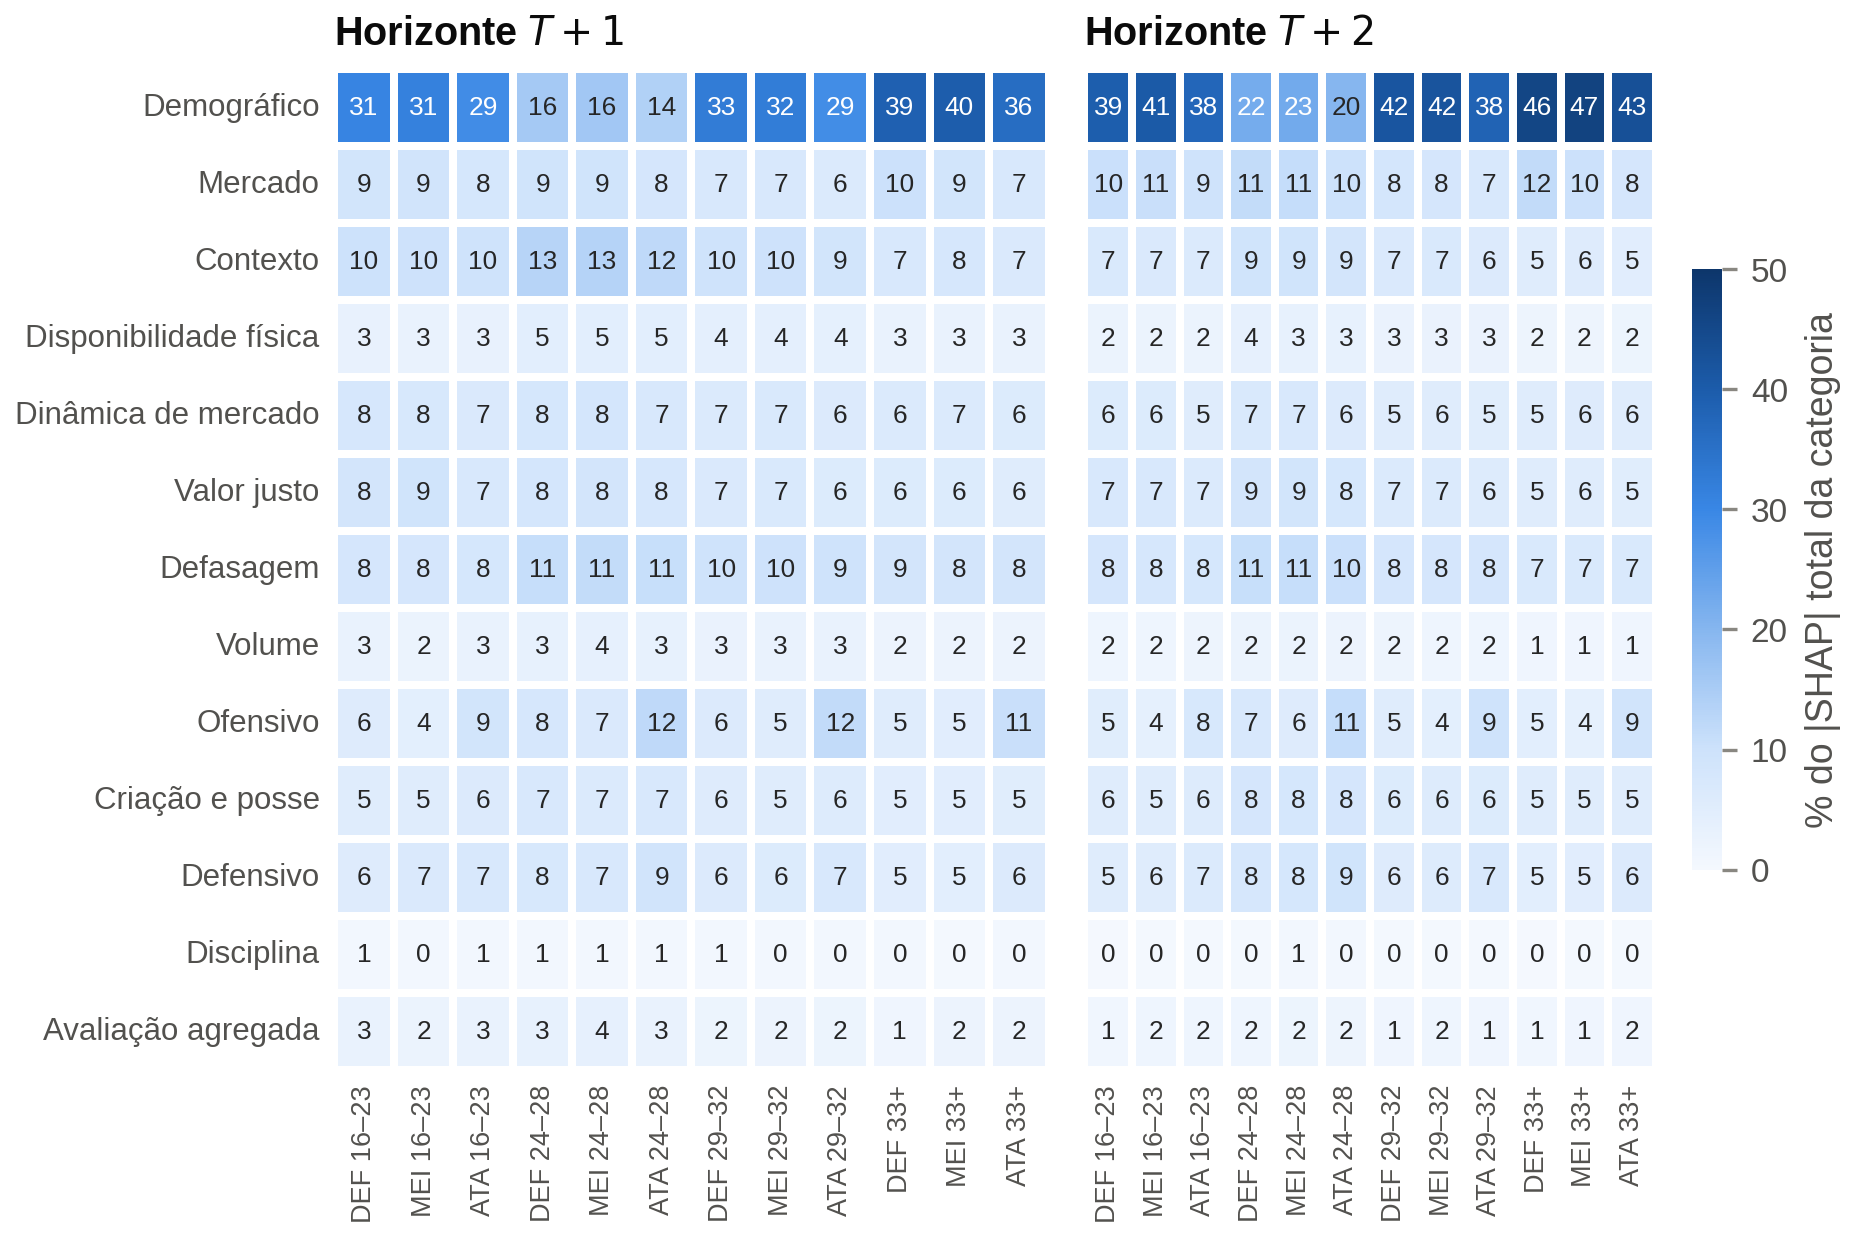
\includegraphics[width=\textwidth]{fig03_grupos_por_categoria.png}
  \fonte{Elaboração própria com dados de FBref, Understat, Sofascore e Transfermarkt.}
\end{figure}

\subsection{Premissa \textit{buy-low} e decisão de compra}

A premissa \textit{buy-low} encontra apoio em $T+1$: no teste, o quintil mais subavaliado pelo \textit{gap} teve mediana de $\Delta V\%$ de −5,9\% (IC 95\%: −12,5\% a 0,0\%), e o mais sobreavaliado, de −20,0\% (−25,0\% a −16,7\%), com correlação parcial de −0,20 entre \textit{gap} e log-retorno, controlada por idade e preço; em $T+2$, o sentido se mantém, mas os intervalos se tocam.
A Tabela~\ref{tab:backtest} apresenta a simulação de carteiras.

\begin{table}[htbp]
  \caption{ROI médio das carteiras, por estratégia, no cenário principal}
  \label{tab:backtest}
  \begin{tabularx}{\textwidth}{Lrrrr}
    \toprule
    Estratégia & $T+1$, todos & $T+1$, €~2–15 mi & $T+2$, todos & $T+2$, €~2–15 mi \\
    \midrule
    Modelo (maior retorno esperado) & 46\% & 40\% & 89\% & 70\% \\
    Modelo prudente (maior percentil 10) & 19\% & 21\% & 54\% & 50\% \\
    10\% mais jovens\textsuperscript{a} & 26\% & 26\% & 55\% & 56\% \\
    \textit{Momentum} & 9\% & 16\% & 15\% & 28\% \\
    Jovens de 16 a 23 anos ao acaso & 6,5\% & 10\% & 22\% & 29\% \\
    Aleatória & −19\% & −19\% & −24\% & −22\% \\
    \bottomrule
  \end{tabularx}
  \fonte{Elaboração própria.}
  \nota{Carteiras com 10\% dos candidatos de cada temporada; custos de 10\% na compra e na venda; atletas sem $V_{T+k}$ valem zero. Médias de seis temporadas em $T+1$ (2019/20 a 2024/25) e de quatro em $T+2$ (2020/21 a 2023/24). \textsuperscript{a} Referência acrescentada após a revelação do teste.}
\end{table}

A carteira do modelo supera todas as alternativas, líquida de custos, e vence a aleatória e o \textit{momentum} nas seis temporadas de $T+1$ (teste do sinal, $p = 0,016$) e nas quatro de $T+2$ ($p = 0,063$), em todos os cenários de custo e de tratamento dos ausentes.
No teste pré-registrado de 2024/25, o ROI foi de 87\%, contra −16\% ao acaso.
O resultado resiste à concentração: sem os três maiores acertos de cada carteira, o ROI sem custos de $T+1$ fica acima de 34\% em todas as temporadas.

Como o objetivo gerencial é decidir quem comprar, as previsões foram também avaliadas como regra de decisão, em análise secundária definida após a revelação do teste (Figura~\ref{fig:regra}).
Cerca de 21\% dos atletas se valorizam o bastante para pagar a operação; o modelo os separa com AUC de 0,82 (IC 95\%: 0,80 a 0,84) em $T+1$ e de 0,83 em $T+2$, e 67\% e 62\% do seu decil superior pagaram a operação, contra praticamente nenhum atleta do decil inferior.

Boa parte dessa separação vem da idade: comprar os 10\% mais jovens já atinge AUC de 0,80 em $T+1$ e de 0,84 em $T+2$.
O modelo supera essa heurística em $T+1$ (+0,020 de AUC, IC 95\% de 0,009 a 0,031) e empata em $T+2$.
Sua contribuição própria aparece no auge da carreira, em que de 39\% a 42\% do seu decil superior pagaram a operação, contra 19\% a 25\% dos mais jovens da faixa; no retorno, em que suas carteiras superam as dos mais jovens em todas as temporadas; e na probabilidade calibrada, confiável em $T+1$ (70\% dos atletas com probabilidade acima de 60\% pagaram a operação) e otimista em $T+2$.

O risco permanece relevante: num orçamento de €~40 milhões, com até seis atletas de €~2 a 15 milhões diversificados por posição e idade, o ROI do modelo em $T+1$ variou de +5\% a +173\% entre as temporadas, com probabilidade de perda de até 43\% nos anos fracos, contra perdas em 73\% a 89\% das carteiras com ordem de compra aleatória.
Além disso, as maiores oportunidades concentram-se em promessas de clubes de elite, cujo $V_T$ dificilmente corresponde ao preço de venda.

Para diretores de futebol e departamentos de \textit{scouting}, portanto, os resultados sugerem usar o modelo para triagem, e não para precificação individual: o decil inferior previsto funciona como lista de exclusão, e o superior concentra oportunidades cuja análise deve combinar o intervalo de 80\%, a diversificação da carteira e o preço efetivo de compra.
O desempenho merece mais peso na avaliação de atletas no auge; entre os veteranos, a idade domina, e pagar por desempenho recente tende a não ser recompensado na revenda.

\begin{figure}[htbp]
  \caption{Desempenho do modelo como regra de compra: acerto das carteiras e calibração da probabilidade de a valorização pagar os custos da operação}
  \label{fig:regra}
  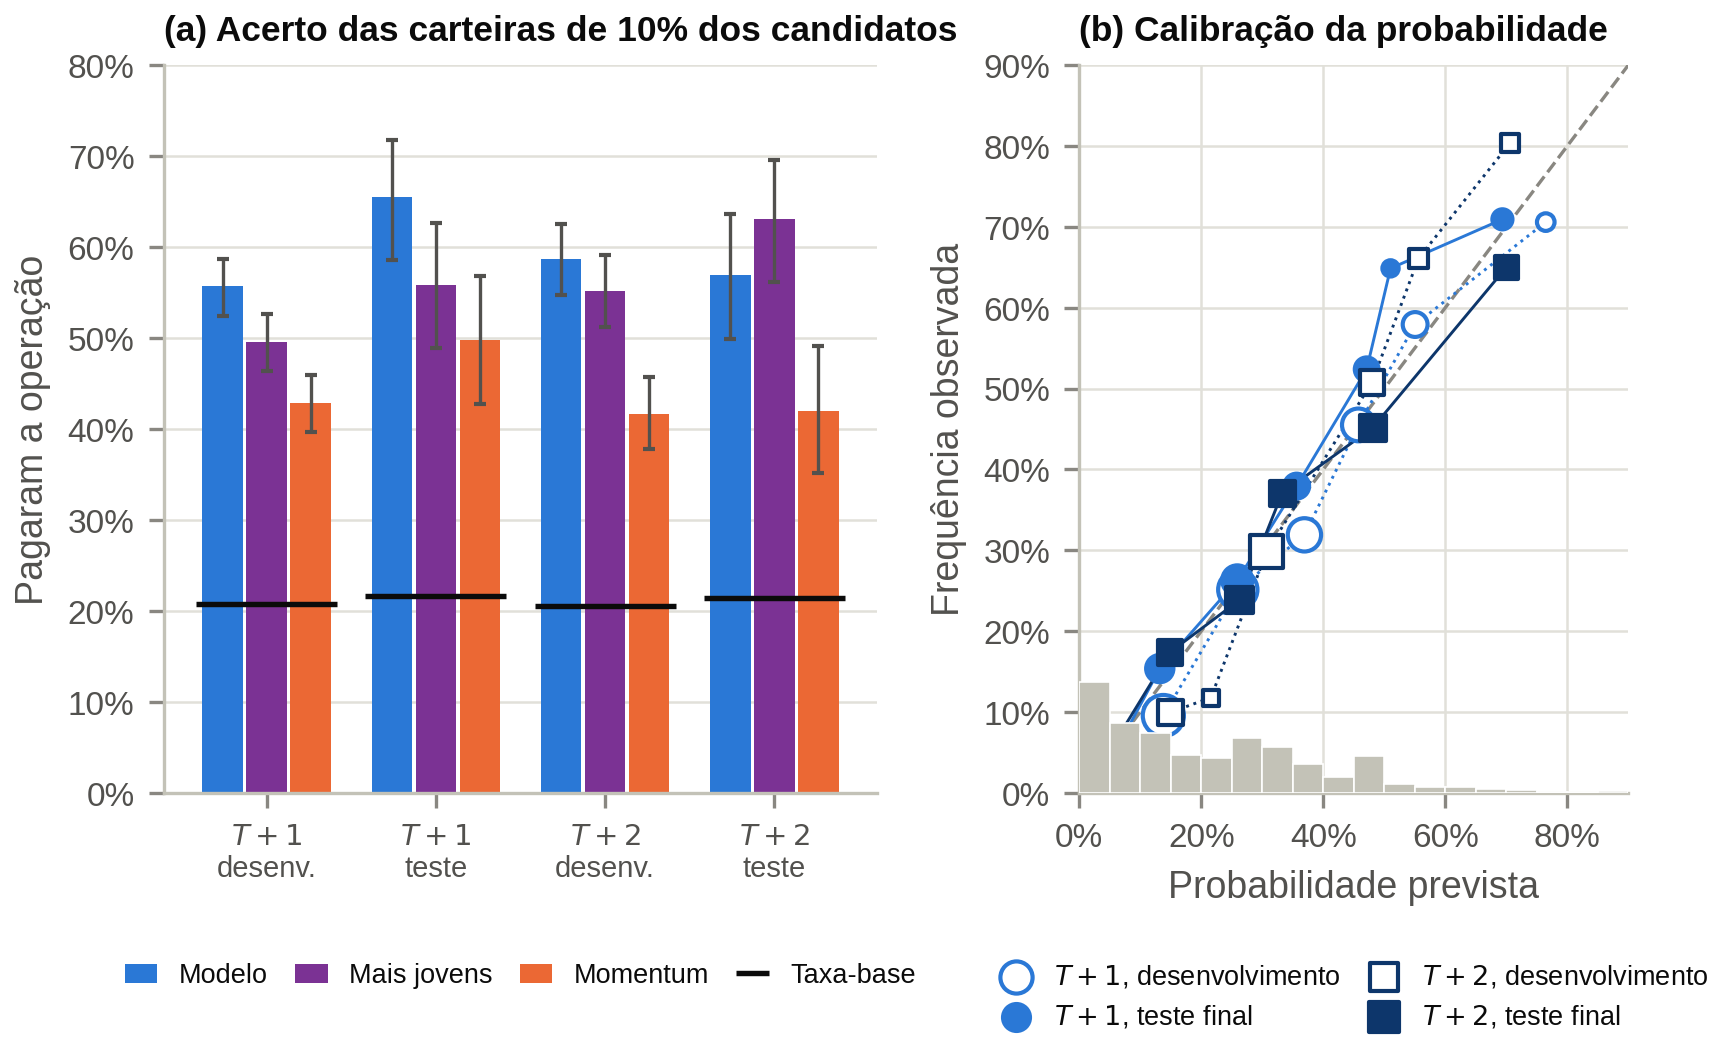
\includegraphics[width=\textwidth]{fig12_regra_de_compra.png}
  \fonte{Elaboração própria com dados de FBref, Understat, Sofascore e Transfermarkt.}
  \nota{Pagar a operação: $\Delta V\%$ acima de 22,2\% (custos de 10\% na compra e na venda). Probabilidade calibrada por regressão isotônica apenas com as temporadas anteriores.}
\end{figure}

\section{Conclusão}

Este artigo investigou em que medida a variação do valor de mercado dos jogadores de linha mais baratos das \textit{Big Five} pode ser prevista uma e duas temporadas à frente.
Num teste temporal pré-registrado, o modelo explicou 33\% da variância do log-retorno em $T+1$ e 37\% em $T+2$, ordenou os atletas de forma consistente e sustentou carteiras que superaram o acaso, o \textit{momentum} e a compra dos mais jovens em todas as temporadas, líquidas de custos.
A resposta à pergunta de pesquisa é afirmativa quanto à ordenação e à decisão, e cautelosa quanto à magnitude: o erro individual permanece alto, e os maiores saltos de valor seguem subestimados.

O estudo mostra que o desempenho em campo agrega informação ao próprio Transfermarkt, sobretudo no auge da carreira, embora a idade seja o principal determinante; que a segmentação em 12 categorias não melhora a previsão; e que previsões de valorização devem ser avaliadas como regra de compra, com limiar derivado dos custos e comparação explícita com a heurística de idade.

Entre as limitações, o valor do Transfermarkt é uma \textit{proxy} do preço, sujeita à inércia dos avaliadores, e o retorno simulado é de valor de mercado, e não de caixa; apenas a temporada 2024/25 é inteiramente independente das decisões de modelagem, e a avaliação como regra de compra foi definida após a revelação do teste; faltam lesões, convocações e histórico contratual; e a amostra é afetada pela revisão de valores da pandemia.
Como trabalhos futuros, recomendam-se a verificação da lista prospectiva emitida para junho de 2027, um novo protocolo pré-registrado com as métricas de decisão, a incorporação de dados contratuais e de lesões e modelos específicos para os saltos extremos de valor.

\printbibliography[heading=referencias]

\end{document}
